\section{Spatial Gaussian Random Fields}
\subsection{Random Fields}
A random field is a set of random variables $\vec{Y}$ that has a distribution function 
\begin{equation} \label{eq:distribution_function}
F(Y(s_1) \leq y_1, \dots , Y(s_n) \leq y_n)
\end{equation} 

for any number for any number $n$, and for any combination of coordinates $s_1$, $\ldots$, $s_n$. A random field has typically some attribute that connects the random variables in $\vec{Y}$. Some examples of such attributes may be physical location, placement in a graph or ordering in time.

Depending on the properties of the distribution function and the setting in which it is defined, we have many different types of random fields, e.g. Markov Random Fields, Gibbs Random Fields and Conditional Random Fields, all of which may again be used with different attributes connecting the variables of the field. 

For this particular project, the main focus will revolve around a random field of type \textit{Gaussian Random Field} (GRF). A GRF is set up so that the variables $\vec{Y}$ is governed by a \textit{Gaussian process}. In addition, the Gaussian process- variance will be assumed to be stationary, meaning that the Gaussian probability distributions of the process is invariant to translations in time or space.

\subsection{Covariance functions} \label{sec:covariance_functions}

For a GRF with equal variance for all associated variables, two of them being $X$ and $\vec{Y}$, we have that the covariance is defined by:
\begin{align*}
\frac{Cov( X, Y )}{\sqrt{Var( X )}\sqrt{Var( Y )}} = \frac{Cov( X, Y )}{\sigma^2} &= Corr(X, Y) \\
\implies  Cov( X, Y ) &= \sigma^2 Corr(X, Y)
\end{align*}
with $\sigma^2$ being the variance parameter of the covariance function. So the covariance of two variables are linear with their pairwise correlation. 

Evidently, by defining a covariance function to use for a Gaussian process, one achieves a covariance with fewer parameters to estimate or set. This simplification is desireable and acceptable for many different models, as we now are down to estimate or set what is typically a couple of parameters compared to estimating $\frac{(n-1)\cdot(n - 2)}{2}$ covariances for a Gaussian process with $n$ variables. In addition, by using a defined covariance function one is then guaranteed that the resulting covariance matrix is a \textit{positive definite matrix} \footnote{Let $M \in \mathcal{R}^n \times \mathcal{R}^n$ with $M = M^T$ be a positive definite matrix. Then, for any $\vec{z} \in \mathcal{R}^n$ we have $\vec{z}^T M \vec{z} \ > \ 0$.}. This further implies the existence of a inverse of the covariance matrix, that's positive definite as well. 

In a spatial GRF setting as this case will use, the associated variables will be linked with a spatial location. The main link will be the Euclidean distance between points, denoted as $d = |s_X - s_Y|$ where $s_A$ is the spatial location for variable A. Combine this with the fact that we have the Gaussian process as time-stationary, the covariance function simplifies to a single-argument function of $d$:
\begin{equation}
Cov(X, Y) = \sigma^2Corr(X, Y) = \sigma^2C(|s_X - s_Y|) = \sigma^2C(d)
\end{equation}

This means the covariance function of our model is \textit{isotropic}, relying solely on distance between variables for its calculation. Whether this simplification is reasonable comes down to model specification. However, in a spatial setting where one is modelling geophysical attributes that only change significantly in time windows of thousands of years, there is a strong argument for defining our covariance in this form. However, covariance functions may also be defined in convenient forms in the case of non-stationarity. In Springer one may find a decent review of covariance functions and methods that allows these to be defined within a non-stationary setting \cite{LeEtAl}. 

For the choice of covariance functions there are many possibilities. A simple function is the exponential correlation function:
\begin{equation*}
C(d) = \sigma^2 \cdot \text{exp}(-\frac{d}{\tau})
\end{equation*}
where $d$ is the Euclidean distance between two stochastic points X and Y in the GRF. $\tau$ is a \textit{range} parameter, describing the intensity in which the distance should affect the correlation. For easy interpretation with the exponential covariancefunction, the distance $d = 3\tau$ is of interest as the resulting correlation is exp$(-3) \approx 0.05$.
The exponential covariance function is derived as a special case of the family of \textit{Mátern covariance functions}. The Mátern covariance functions is defined in a stationary form, with distance $d$, range parameter $\tau$ and degrees of freedom $\nu$, as:
\begin{equation} \label{eq:matern_function}
C_{\nu}(d) = \sigma^2 \frac{2^{1-\nu}}{\Gamma(\nu)}\bigg( \frac{d}{\tau} \bigg)^{\nu} K_{\nu} \bigg( \sqrt{2\nu}\frac{d}{\tau} \bigg)
\end{equation}
where $K_{\nu}$ is the modified Bessel function of the second kind. The covariance functions obtained from the Mátern family makes sample paths of an associated Gaussian process become $\nu - 1$ differentiable. The equation in (\ref{eq:matern_function}) is seemingly a complicated affair to evaluate, but it is reducable to convenient forms for many choices of $\nu$. Three of them are:
\begin{align} \label{eq:covariance_functions}
\begin{split}
\nu = \frac{1}{2}: \quad C_{\frac{1}{2}}(d) &= \sigma^2\text{exp}(-\frac{d}{\tau}) \\
\nu = \frac{3}{2}: \quad C_{\frac{3}{2}}(d) &= \sigma^2 \bigg(1  +
\frac{\sqrt{3}d}{\tau} \bigg) \text{exp}(-\frac{\sqrt{3}d}{\tau}) \\
\nu = \frac{5}{2}: \quad C_{\frac{5}{2}}(d) &= \sigma^2 \bigg(1  +
\frac{\sqrt{5}d}{\tau} + \frac{5d^2}{3\tau^2}\bigg) \text{exp}(-\frac{\sqrt{5}d}{\tau})
\end{split}
\end{align}
These covariancefunctions are presented in figure (\ref{fig:correlation_tau5}). The exponential covariance function is recognized as the Mátern covariance function with d.o.f. $\nu = \frac{1}{2}$. This again implies that we will not have differentiable sample paths when taken from a Gaussian process using this covariance function, something that's illustrated in the figure (\ref{fig:sample_path_simple}).  

\begin{figure}[p]
     \centering
     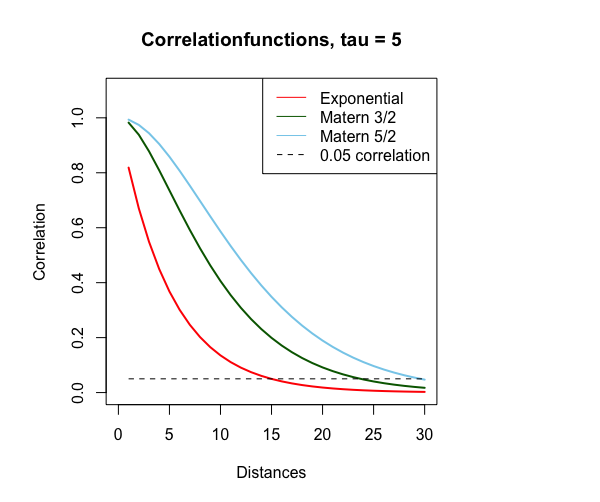
\includegraphics[width=0.8\linewidth]{figurer/correlation_tau5.png}
     \caption{Correlation with $\tau = 5$ as function of distance.}
     \label{fig:correlation_tau5}
\end{figure}
\begin{figure}[p]	
     \centering
     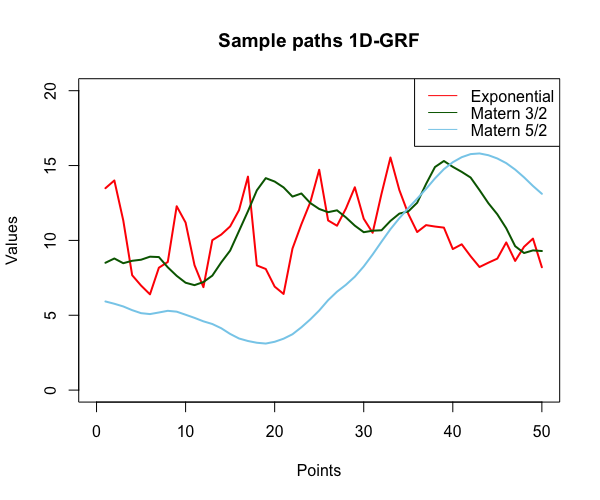
\includegraphics[width=0.8\linewidth]{figurer/sample_paths_1d.png}
	 \caption{Sample paths from a 1D-GRF, mean $\mu = 10$, variance $\sigma^2 = 10$ and range $\phi = 5$.}
	 \label{fig:sample_path_simple}
\end{figure}

\subsection{Gaussian processes} \label{sec:gaussian_processes}
Associated with every GRF is a underlying Gaussian process detailing the distributions of the variables defining the field. The fundamental characterization of such a process is that all finitie-dimensional joint distributions for the variables of the process is multivariate normally distributed (MVN), and especially that each variable is normally distributed. Being distributed as a MVN, a Gaussian process is completely determined by its mean and covariance functions \cite{RasmussenEtAl}. Thus, the mean and covariance functions of a process are often a focus point in dealing with a Gaussian process. 

Amongst the many favourable properties of MVN distributions, we have that the best predictor for an unobserved variable in a Gaussian process is linear function of the observed variables. The predictor being a linear function of MVN distributed variables, the predictor as well is MVN distributed with an adjusted mean and covariance.

More precisely, if $\begin{bmatrix} \vec{A} \\ \vec{B} \end{bmatrix}$ is a vector of $n$ stochastic variables associated with a Gaussian process, meaning $\begin{bmatrix} \vec{A} \\ \vec{B} \end{bmatrix}$ has a distribution on the form of $\mathcal{MVN}(\begin{bmatrix} \mu_{\vec{A}} \\ \mu_{\vec{B}} \end{bmatrix}, \begin{bmatrix} \Sigma_{\vec{A}\vec{A}} & \Sigma_{\vec{A}\vec{B}} \\ \Sigma_{\vec{B}\vec{A}} & \Sigma_{\vec{B}\vec{B}} \end{bmatrix})$, where $\Sigma_{\vec{A}\vec{B}} = \Sigma_{\vec{B}\vec{A}}^T$ denotes the covariance between the variables in $\vec{A}$ versus the variables in $\vec{B}$.  Given $\vec{B}$, we have exact results for the best linear predictor. $P(\vec{A} | \vec{B} = \vec{b})$ will then be $MVN$, with corrected mean $\mu_{\vec{A} | \vec{B}}$ and variance $\Sigma_{\vec{A} | \vec{B}}$ as:
\begin{equation}\label{eq:gaussian_conditional_expectancy} 
\mu_{\vec{A} | \vec{B}} = \mu_{\vec{A}} + \Sigma_{\vec{A}\vec{B}}\cdot \Sigma_{\vec{B}\vec{B}}^{-1}\big( \vec{b} - \mu_{\vec{B}} \big) 
\end{equation}
\begin{equation}\label{eq:gaussian_conditional_variance}
\Sigma_{\vec{A} | \vec{B}} = \Sigma_{\vec{A}\vec{A}} - \Sigma_{\vec{A}\vec{B}} \cdot \Sigma_{\vec{B}\vec{B}}^{-1} \cdot \Sigma_{\vec{B}\vec{A}} 
\end{equation}

In an informal setting, one may interpret this as a linear smoothing of the parameters for the MVN distribution of $\vec{A}$. Especially it's worth noting that since the covariance matrix $\Sigma_{\vec{B}\vec{B}}$ is positive definite, its inverse is as well, meaning that the diagonal entries of $\Sigma_{\vec{A}\vec{B}} \cdot \Sigma_{\vec{B}\vec{B}}^{-1} \cdot \Sigma_{\vec{B}\vec{A}}$ are all greater or equal to zero. As the variance of each variable in $P(\vec{A} | \vec{B} = \vec{b})$ are the diagonal elements of $\Sigma_{\vec{A}|\vec{B}}$, we have that the elementwise variance after conditioning on $\vec{B}$ is lower or equal than with no conditioning: 
\begin{equation}
\Sigma_{\vec{A}|\vec{B}} = \Sigma_{\vec{A}\vec{A}} - \Sigma_{\vec{A}\vec{B}} \cdot \Sigma_{\vec{B}\vec{B}}^{-1} \cdot \Sigma_{\vec{B}\vec{A}}
\implies \Sigma_{\vec{A}|\vec{B}}[i, \ i]  \leq \Sigma_{\vec{A}\vec{A}}[i, \ i] \quad  i = 1, \dotsc, n.
\end{equation}
where $\Sigma_{\vec{A}\vec{A}}[i, \ i]$ denotes the entry at index $(i, i)$ in the matrix. As the matrices $\Sigma_{\vec{A}\vec{B}}$ and $\Sigma_{\vec{B}\vec{B}}^{-1}$ consists solely of positive real numbers, the equality will only hold in the case that there are no correlation between variable $i$ of $\vec{A}$ and all the variables in $\vec{B}$. Intuitively, this makes sense as then the variable $\vec{A}_i$ have no relation to the variables in $\vec{B}$. 

As an example, three predictions using these results have been plotted in figures (\ref{fig:prediction_exp5}), (\ref{fig:prediction_325}) and (\ref{fig:prediction_525}). The actual processes shown in red are Gaussian processes in a 1D-GRF with spatial points $s \in \{1,\dots, 50\}$. A common set of parameters are set with mean $\mu = 10$, variance $\sigma^2 = 10$ and range $\tau = 5$. Data were sampled in all cases as noise-free at location $s \in \{8, 25, 43\}$. The difference is which covariancefunction that's used to simulate the process in the three figures.

\begin{figure}[p]
\minipage{0.48\textwidth}
	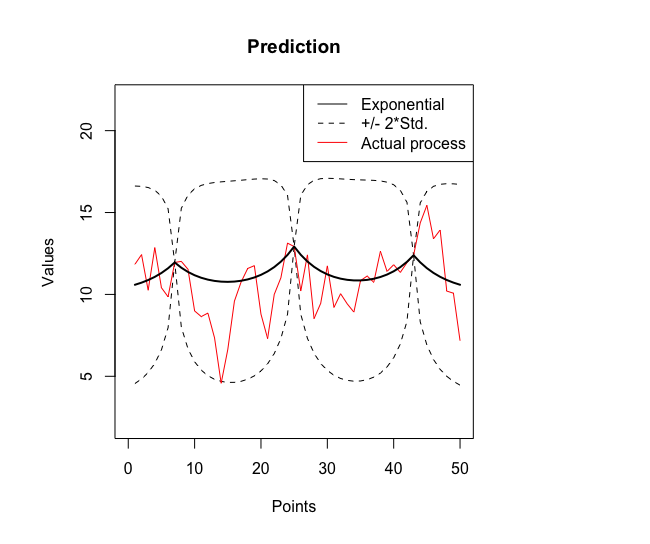
\includegraphics[width=1.4\linewidth]{figurer/prediction_exp5.png}
  	\caption{Predictions with an Exponential covariancefunction}	
  	\label{fig:prediction_exp5}	
	\endminipage\hfill
	\minipage{0.48\textwidth}
  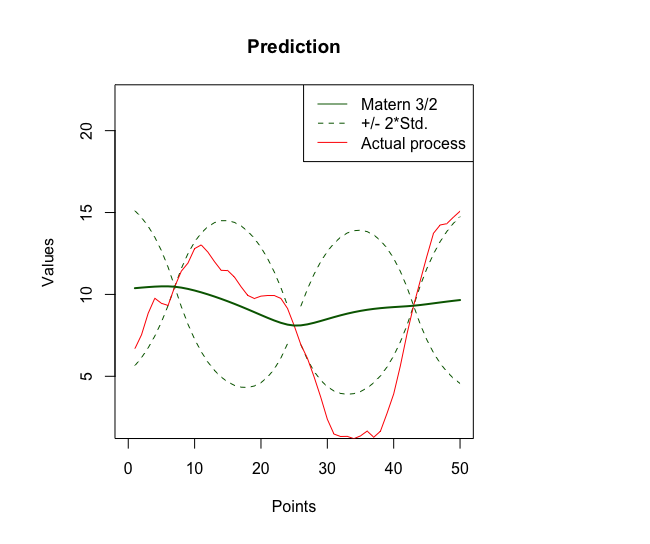
\includegraphics[width=1.4\linewidth]{figurer/prediction_325.png}
	\caption{Predictions with Matern covariancefunction, d.o.f. $\nu = \frac{3}{2}$}
	\label{fig:prediction_325}
\endminipage
\end{figure}
\begin{figure}
	\centering
	\hspace{60pt}
	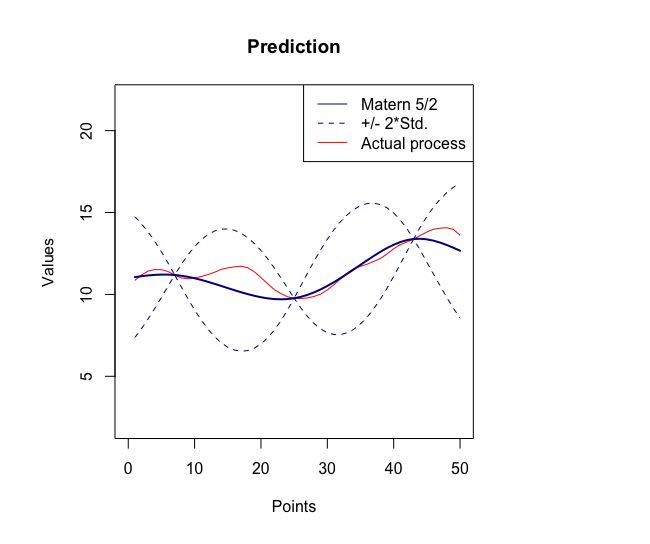
\includegraphics[width=0.8\linewidth]{figurer/prediction_525.png}
    \caption{Predictions with Matern covariancefunction, d.o.f. $\nu = \frac{5}{2}$}
    \label{fig:prediction_525}
\end{figure}

Evidently from the easy to achieve posterior distribution, when dealing with a Gaussian process it would be favourable to have well-defined expressions for its mean and covariance. Regarding the process-covariance, covariancefunctions has been mentioned as a possible solution. In this project results will be presented for all the covariancefunctions defined in equation (\ref{eq:covariance_functions}).

\subsection{Generalized least squares}

The trendfunction is another matter. As we are unaware of any data in the grid that may be related to the trend of the GRF model, the better option that is left is to estimate the trend based on the curent data aqcuisition. The trendfunction is defined as a polynomial function of spatial location on the form $\mu(\vec{s}) = X(\vec{s})\vec{\beta}$, where X is a design matrix corresponding to the locations $\vec{s}$ and $\vec{\beta}$ is vector of coefficients. By doing so we may utilize results from the theory of \textit{Generalized Least Squares} (GLS) in the estimation of trend. One particular advantage of using GLS is that we are guaranteed by the Gauss-Markov Theorem that the GLS estimates is the \textit{Best Linear Unbiased Estimator} (BLUE) for the vector of coefficients $\vec{\beta}$. 

One of two caveats with using GLS estimates is that one still need to specify the polynomial trendfunction to fit the data, meaning there's still a selection process. As the trendfunction is to specified by spatial location for this case, one must face the second caveat. The GLS estimates are the BLUE only for the data and their associated spatial location used in the estimation, giving no guarantee for the prediction of data not part of the estimates. By this, the trendfunction will be selected to be a polynomial of lower order with simple interaction between easting- and northing-coordinates, i.e. for a variable with coordinates $(s_E, s_N)$:
\begin{equation} \label{eq:formula}
X(s_E, s_N)\vec{\beta} = \beta_0 + s_{E} \cdot \beta_1 + s_{N} \cdot \beta_2 + s_{E} \cdot s_{N} \cdot \beta_4 
\end{equation} 
This has been chosen as an prediction far away from the sample data will typically be over- or underpredicted by an unacceptable amount using a higher-order polynomial. This is due to the covariates of said polynomial will be fitted to the data that has been sampled, which in this case will be done mainly by a specified design of low regularity. In sampling designs with high regularity over the field, this is effect is handled as then the estimation will try to adapt to grid points that has a regular distance between each other. An example of this issue is shown in figures (\ref{fig:gls_simple}) and (\ref{fig:gls_quadratic}), where a proposed sampling design is used two different polynomial distributions are fitted. 

When the samples are drawn from a distribution with known correlation matrix $\Omega = \sigma^2 \cdot W$, with $\sigma^2$ as a constant finite variance parameter and $W$ the correlation matrix, the estimates of $\vec{\beta}$ converge in distribution to a MVN, or more precisely
\begin{equation}
\hat{\vec{\beta}} \xrightarrow[]{d} \mathcal{MVN} \big( \ \vec{\beta}, \ (X^T \Omega^{-1} X)^{-1} \big)
\end{equation}
where $X$ denotes the associated design matrix of the samples used to estimate the trend. In figures(\ref{fig:gls_simple}) and (\ref{fig:gls_quadratic}) the GLS estimation has been used on the data acquired at the sample path indicated by the black line. The data is from the case data, modelled with an Exponential covariancefunction. A GLS estimate was fitted with both a simple linear formula of equation (\ref{eq:formula}) and a quadratic formula of equation (\ref{eq:formula}) $+ s_{E}^2 \cdot \beta_5 + s_{N}^2 \cdot \beta_6$. The effect of overestimation in the fitted modell is not so obvious as the grid size is fairly low, but you can see that the quadratic formula's variance increases rapidly as we move towards the outer edges, away from the sampled data. 

\begin{figure}[p]
     \centering
     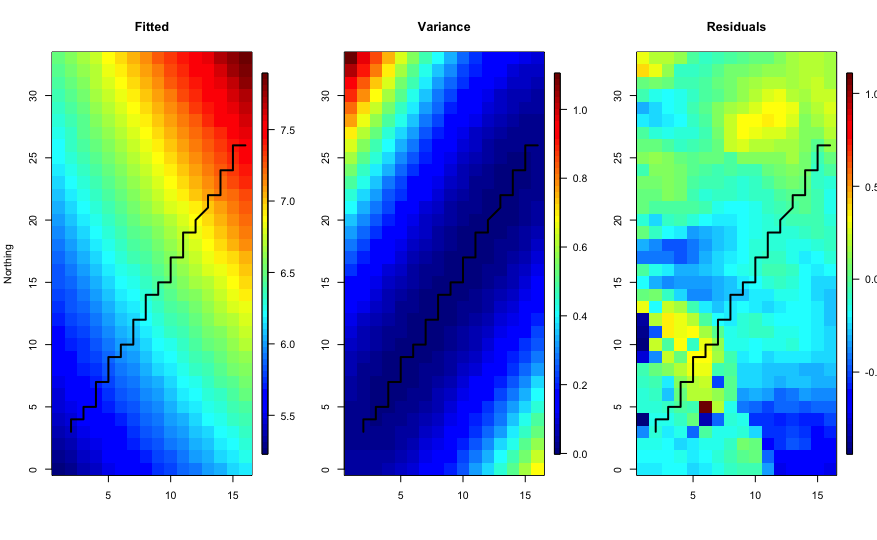
\includegraphics[width=1\linewidth]{figurer/gls_simple.png}
     \caption{GLS fit by perfect data from the black line. Linear model with interaction.}
      \label{fig:gls_simple}
\end{figure}
\begin{figure}[p]
     \centering
     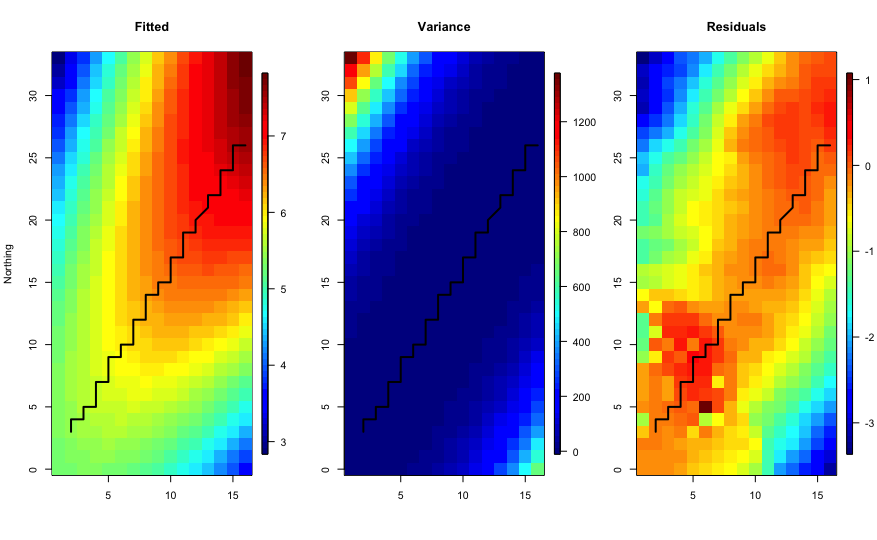
\includegraphics[width=1\linewidth]{figurer/gls_quadratic.png}
	 \caption{GLS fit by perfect data from the black line. Quadratic model with interaction.} 
	 \label{fig:gls_quadratic}
\end{figure}

\subsection{Hierarchical model} \label{model:hm}
Apart from specifying the design of the GRF, it's preferable to clearly relate the GRF and its attributes to the data acquisition. One may also specify any noise in the data acquisition in a precise matter. One common way of specifying this relation is to describe the data acquisition and gaussian process in a hierarchical model. An advantage of doing so is the lack of restriction that the model presents on the parameters of the model. In the case of Bayesian modelling, we also have the advantage of clearly connecting the different levels through the updating posterior distributions that are of interest, encapsulating the uncertainty of the different levels in an easy to interpret way \cite{LeEtAl}.  

A hierarchical model divides the spatial design model 
into three parts: 
\begin{itemize}
\item Data model - Describes the relation between process and datasampling
\item Process model - Describes the model properties of the GRF 
\item Prior model - Priors used in the case of Bayesian modelling of parameters
\end{itemize}


An example with fixed parameters, i.e. without a "Prior model", is given here. Denoting $\vec{Z}$ as the sampled data, $\vec{Y}$ as the underlying GP and parameters $\mu, \tau, \sigma^2, \phi$:
\begin{align*}
\textbf{Data model: } \vec{Z}(\vec{s}) &\sim \mathcal{MVN}\big(F(\vec{s}) \cdot \vec{Y},  \phi^2I_{n \times n}\big) \\
\textbf{Process model: } \vec{Y} &\sim \mathcal{MVN}\big( \vec{\mu}, \ C_{\vec{Y}} ( D, \sigma^2, \tau) \big)
\end{align*}
where $\vec{s} \in \mathcal{R}^n \times \mathcal{R}^2$ is the matrix of coordinates for the $n$ variables in question, $D$ denotes a symmetric $n \times n$ matrix of distances between the points in the field, F is a matrix indicating sampling of data and $C_{\vec{Y}}(\dots)$ the chosen covariance function. In this case $\rho$ indicates the covariance that arises due to the prosess, whilst $\epsilon$ may be interpreted as possible noise that arises when the data is acquired. In this paper, $\epsilon$ will be treated as a fixed constant and not a stochastic variable within the Bayesian framework. A motivation for this is that $\epsilon$ models the knwon uncertainty of measurement-equipment.

By using the linearity property of Gaussian variables, we may write the models as linear combinations of their means and covariances, i.e. 
\begin{align} \label{hm:linear_model}
\begin{split}
\textbf{Data model: } \vec{Z}(\vec{s}) &= F(\vec{s}) \cdot \vec{Y} + \vec{\epsilon}, \quad \vec{\epsilon} \sim \mathcal{MVN} \big(\vec{0},\phi^2I(\vec{s}) \big) \\
\textbf{Process model: } \vec{Y} &= \vec{\mu} + \rho, \quad \rho \sim \mathcal{MVN} \big(\vec{0}, \ C_Y(D, \sigma^2, \tau ) \big)
\end{split}
\end{align}
This is a unique property of models with a GRF and Gaussian distributed noise and is of no difference compared to the first model. Sample paths for a model of this type was model is shown in (\ref{fig:sample_path_simple}), where $F(\vec{s})$ is set to be $I_{n \times n}$ for the $n$ variables in the field, i.e. perfect sampling of the field.

\subsubsection{Deriving the posterior GRF}
The ultimate goal of the analysis is to provide a result for the posterior distribution of the underlying Gaussian process, given some sample data, that is $P \big( \vec{Y} | \vec{Z}(\vec{s_0}) \big)$ where $\vec{s}$ denotes the whole coordinates of the whole field and $\vec{s_0}$ denotes the coordinates of samples obtained. This distribution is derived as 
\begin{align*}
\begin{split}
P \big( \vec{Y} | \vec{Z}(\vec{s_0}) \big) &= \int \int P \big( \vec{Y}, \sigma^2, \tau | \ \vec{Z}(\vec{s_0}) \big) \ d\sigma^2 \ d\tau \\
&= \int \int P \big( \vec{Y} | \vec{Z}(\vec{s_0}), \sigma^2, \tau \big) \cdot P\big( \sigma^2, \tau | \vec{Z}(\vec{s_0}) \big) \ d\sigma^2 \ d\tau 
\end{split}
\end{align*}
Further, we use Bayes Theorem 
\begin{align}\label{eq:posterior_prior}
\begin{split}
P\big( \sigma^2, \tau | \vec{Z}(\vec{s_0}) \big) &\propto P\big( \vec{Z}(\vec{s_0}) | \sigma^2, \tau \big) \cdot P\big( \sigma^2, \tau \big) \\[5pt]
&\propto P\big( \vec{Z}(\vec{s_0}) | \sigma^2, \tau \big) \cdot P\big( \sigma^2 \big) \cdot P\big( \tau \big) \\[10pt]
\implies P\big( \sigma^2, \tau | \vec{Z}(\vec{s_0}) \big) &= \frac{P\big( \vec{Z}(\vec{s_0}) | \sigma^2, \tau \big) \cdot P\big( \sigma^2 \big) \cdot P\big( \tau \big)}{\int \int P\big( \vec{Z}(\vec{s_0}) | \sigma^2, \tau \big) \cdot P\big( \sigma^2 \big) \cdot P\big( \tau \big) d\sigma^2 d\tau}
\end{split}
\end{align}
This implies that 
\begin{equation}\label{eq:grf_posterior}
\hspace*{-0.1cm}
P \big( \vec{Y} | \vec{Z}(\vec{s_0}) \big) = \int \int P \big( \vec{Y} | \vec{Z}(\vec{s_0}), \sigma^2, \tau \big) \cdot \frac{P\big( \vec{Z}(\vec{s_0}) | \sigma^2, \tau \big) \cdot P\big( \sigma^2 \big) \cdot P\big( \tau \big)}{\int \int P\big( \vec{Z}(\vec{s_0}) | \sigma^2, \tau \big) \cdot P\big( \sigma^2 \big) \cdot P\big( \tau \big) d\sigma^2 d\tau} \ d\sigma^2 \ d\tau
\end{equation}

An exact analytical result for the posterior found in both (\ref{eq:posterior_prior}) and (\ref{eq:grf_posterior}) may be found under the with the appropriate priors, but to acommodate any type of prior from a probability distribution, the integrals is approximated by a simple numerical procedure. This is done by discretizing the domain of $\sigma^2$ and $\tau$ and summing over the discretizied values with some weight $\Delta$ for each discretization to ensure normalization, giving an approximation as
\begin{align*}
\begin{split}
P \big( \vec{Y} | \vec{Z}(\vec{s_0}) \big) &\approx \frac{1}{\Pi}\sum_{\tau_i}^{n_{\tau}} \sum_{\sigma^2_j}^{n_{\sigma}} P \big( \vec{Y} | \vec{Z}(\vec{s_0}), \sigma^2_j, \tau_i \big) \cdot P\big( \vec{Z}(\vec{s_0}) | \sigma^2_j, \tau_i \big) \cdot P\big( \sigma^2_j \big) \cdot P\big( \tau_i \big) \cdot \Delta_{ij}
\end{split}
\end{align*}
With $\Pi = \sum_{\tau_i}^{n_{\tau}} \sum_{\sigma^2_j}^{n_{\sigma}} P\big( \vec{Z}(\vec{s_0}) | \sigma^2_j, \tau_i \big) \cdot P\big( \sigma^2_j \big) \cdot P\big( \tau_i \big) \cdot \Delta_{ij}$ as the normalizing constant.

For this integration to be performed, four distributions need to be defined: $P\big( \sigma^2_j \big)$ and $P\big( \tau_i \big)$ are priors given by the model, $P\big( \vec{Z}(\vec{s_0}) | \sigma^2_j, \tau_i \big)$ is known MVN by the model specification and lastly we have that $P \big( \vec{Y} | \vec{Z}(\vec{s_0}), \sigma^2_j, \tau_i \big)$ is MVN by the results presented in section (\ref{sec:gaussian_processes}) with $\vec{Y}$ as $A$ and $\vec{Z}(\vec{s_0})$ as $B$.

When performing the numerical integration, it is noted that it's the mean and variance of $P\big( \sigma^2, \tau | \vec{Z}(\vec{s_0}) \big)$ that's of relevance for the predictions. By similar arguments as above, one gets:
\begin{align}\label{eq:expected_variance_grf_posterior}
\begin{split}
\mathbf{E} \big( \vec{Y} | \vec{Z}(\vec{s_0}) \big) & \approx \frac{1}{\Pi}\sum_{\tau_i}^{n_{\tau}} \sum_{\sigma^2_j}^{n_{\sigma}} \Delta_{ij} \cdot \mathbf{E} \big( \vec{Y} | \vec{Z}(\vec{s_0}), \sigma^2_j, \tau_i \big) \cdot P\big( \vec{Z}(\vec{s_0}) | \sigma^2_j, \tau_i \big) \cdot P\big( \sigma^2_j \big) \cdot P\big( \tau_i \big) \\
\mathbf{Var} \big( \vec{Y} | \vec{Z}(\vec{s_0}) \big) & \approx \frac{1}{\Pi}\sum_{\tau_i}^{n_{\tau}} \sum_{\sigma_j^2}^{n_{\sigma}} \Delta_{ij} \cdot \mathbf{Var} \big( \vec{Y} | \vec{Z}(\vec{s_0}), \sigma^2_j, \tau_i \big) \cdot P\big( \vec{Z}(\vec{s_0}) | \sigma^2_j, \tau_i \big) \cdot P\big( \sigma^2_j \big) \cdot P\big( \tau_i \big) \\\end{split}
\end{align}
with $\Pi$ defined as before. The expressions of $\mathbf{E} \big( \vec{Y} | \vec{Z}(\vec{s_0}), \sigma^2, \tau \big)$ and $\mathbf{Var} \big( \vec{Y} | \vec{Z}(\vec{s_0}), \sigma^2, \tau \big)$ is given in (\ref{eq:gaussian_conditional_expectancy}) and (\ref{eq:gaussian_conditional_variance}).

